\documentclass[12pt, oneside]{article}
\usepackage[letterpaper, margin=1in, headsep=0.5in, left=0.3in, right=2.5in]{geometry}
\usepackage[english]{babel}
\usepackage[utf8]{inputenc}
\usepackage{amsmath}
\usepackage{amsfonts}
\usepackage{amssymb}
\usepackage{tikz}
\usepackage{yhmath}
\usetikzlibrary{quotes, angles}
\usepackage{graphicx}
\usepackage{enumitem}
\usepackage{multicol}

\newif\ifmeta
\metatrue %print standards and topics tags

\title{Regents Geometry}
\author{Chris Huson}
\date{May 2022}

\usepackage{fancyhdr}
\pagestyle{fancy}
\fancyhf{}
\renewcommand{\headrulewidth}{0pt} % disable the underline of the header
\raggedbottom

%\fancyhead[LE]{\thepage}
\fancyhead[RO]{Name:}
\fancyhead[LO]{BECA / Dr. Huson / Geometry Regents Mixed Review}
\cfoot{\thepage}

\begin{document}
\subsubsection*{11.15 Similarity ratios}
\begin{enumerate}[itemsep=1.2cm]
\item In the diagram below of right triangle $AED$, $\overline{BC} \parallel \overline{DE}$.
    \begin{center}
      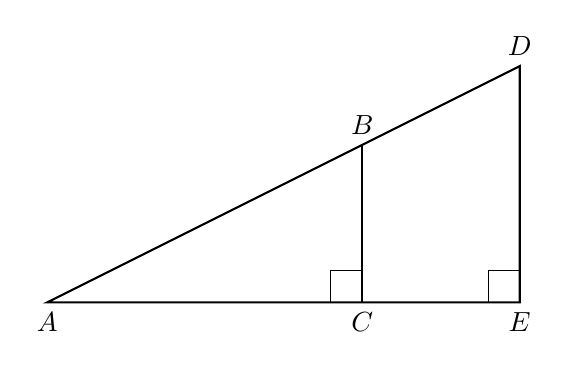
\begin{tikzpicture}[scale=1]
        \draw [-, thick] (0,0) node[below]{$A$}--
        (6,0) node[below]{$E$}--
        (6,3) node[above]{$D$}--cycle;
        \draw [thick] (4,0) node[below]{$C$}--
        (4,2) node[above]{$B$};
        \draw (4,0) ++(-0.4,0)--++(0,0.4)--++(0.4,0);
        \draw (6,0) ++(-0.4,0)--++(0,0.4)--++(0.4,0);
      \end{tikzpicture}
    \end{center} 
    Which statement is always true?
    \begin{multicols}{2}
      \begin{enumerate}[itemsep=0.25cm]
        \item $\displaystyle \frac{AC}{BC} = \frac{DE}{AE}$
        \item $\displaystyle \frac{AB}{AD} = \frac{BC}{DE}$ 
        \item $\displaystyle \frac{AC}{CE} = \frac{BC}{DE}$
        \item $\displaystyle \frac{DE}{BC} = \frac{DB}{AB}$
      \end{enumerate}
    \end{multicols}

\item Determine and state an equation of the line perpendicular to the line\\ $5x-4y=10$ and passing through the point $(5,12)$.

\item What is the equation of a circle whose diameter is $\overline{AB}$ with $A(2,-1)$ and $B(8,7)$?
    \begin{flushright}
      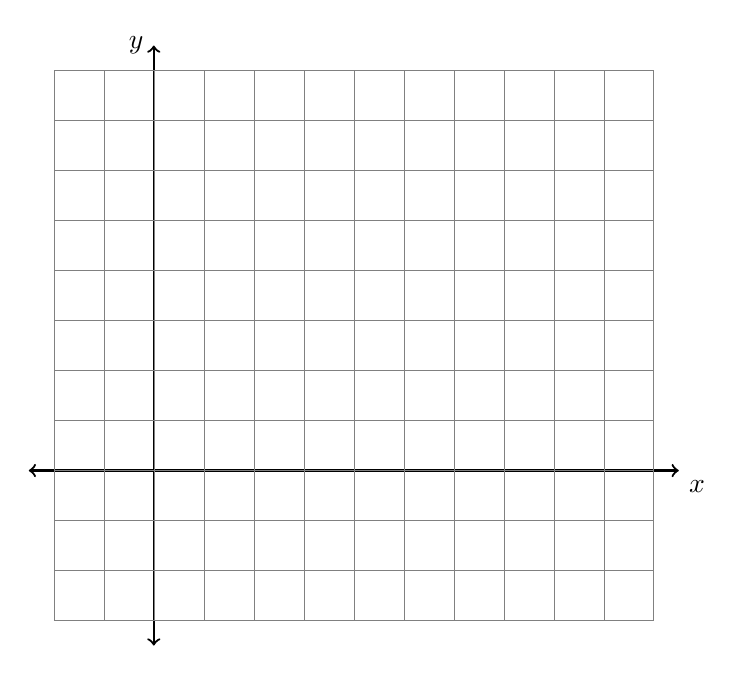
\begin{tikzpicture}[scale=.635]
        \draw [thick, <->] (-2.5,0) -- (10.5,0) node [below right] {$x$};
        \draw [thick, <->] (0,-3.5)--(0,8.5) node [left] {$y$};
        \draw [help lines] (-2,-3) grid (10,8);
      \end{tikzpicture}
    \end{flushright}

\newpage
\item Lou has a solid clay brick in the shape of a rectangular prism with a length of 8 inches, a width of 3.5 inches, and a height of 2.25 inches. If the clay weighs 1.055 oz/in$^3$, how much does Lou's brick weigh, to the nearest ounce?

\item From a point on the ground one-half mile from the base of a historic monument, the angle of elevation to its top is $11.87^\circ$. To the nearest foot, what is the height of the monument? (1 mile = 5280 feet)

\item The coordinates of the endpoints of directed line segment $ABC$ are $A(-8,7)$ and $C(7,-13)$. If $AB:BC = 3:2$, what are the coordinates of $B$?

\item In right triangle $ABC$, $m\angle C=90^\circ$ and $AC \ne BC$. Which trigonometric ratio is equivalent to $\sin B$?
\begin{multicols}{2}
  \begin{enumerate}
    \item $\cos A$
    \item $\cos B$
    \item $\tan A$
    \item $\tan B$
  \end{enumerate}
\end{multicols}

\item Line segment $CD$ is the altitude drawn to hypotenuse in right
triangle $ECF$. If $EC=10$ and $EF=24$, then, to the \emph{nearest
tenth}, $ED$ is what length?

\end{enumerate}
\end{document}
  